\documentclass{beamer}
\usepackage[utf8]{inputenc}
% \usepackage[T1]{fontenc}
% \usepackage[english]{babel}
\usepackage{wrapfig}
\usepackage{verbatim}
\usepackage{ mathrsfs }
\usepackage{dsfont}
\usepackage{amssymb}
\usepackage{amsmath}
\usepackage{amsthm}
\usepackage{graphicx}
\usepackage{lmodern}
\usepackage{float}
\usepackage{listings}
\usepackage{hyperref}
\usepackage{array}
\usepackage{multirow}
\usepackage{caption}
\usepackage{subcaption}
\usepackage{tikz}
\usetikzlibrary{positioning} 
\usetheme{Madrid}
\DeclareMathOperator*{\argmin}{argmin}
\DeclareMathOperator*{\argmax}{argmax}

\title{Inferring the underlying network of diffusion}

\begin{document}

\begin{frame}
\titlepage
\begin{figure}
    \centering
    \includegraphics[scale = 0.5]{EPFL_Todai.jpg}
\end{figure}
\begin{tabular}{l}
     Supervisors :  \\
     Prof. Friedrich Eisenbrand\\
     Prof. Iwata Satoru\\
     Dr. Tasuku Soma
\end{tabular}
\hfill
\begin{tabular}{l}
     Student : \\
     Joachim Moussalli
\end{tabular}
\end{frame}

\begin{frame}{Table of Contents}
\tableofcontents
\end{frame}
\section{Introduction}
\begin{frame}{Motivation}
\begin{columns}
\column{0.5\textwidth}
(Fake) News
\column{0.5\textwidth}
\begin{figure}
    \centering
    \includegraphics[scale = 0.1]{FakeNews.jpg}
\end{figure}
\end{columns}

\begin{columns}
\column{0.5\textwidth}
Marketing
\column{0.5\textwidth}
\begin{figure}
    \centering
    \includegraphics[scale = 0.1]{Iphone.jpg}
\end{figure}
\end{columns}

\begin{columns}
\column{0.5\textwidth}
Diseases
\column{0.5\textwidth}
\begin{figure}
    \centering
    \includegraphics[scale = 0.1]{diseases.jpg}
\end{figure}
\end{columns}
\end{frame}
\begin{frame}{Problem- Underlying network}
\begin{figure}
\begin{subfigure}{.4\textwidth}
    \centering
    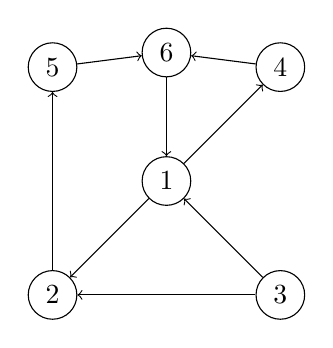
\begin{tikzpicture}[roundnode/.style = {circle, draw=black}]
     \node[roundnode] (1) {1};
     \node[roundnode] (2) [below left=of 1]{2};
     \node[roundnode] (3) [below right=of 1]{3};
     \node[roundnode] (5) [above left=of 1]{5};
     \node[roundnode] (4) [above right=of 1]{4};
     \node[roundnode] (6) [above=of 1]{6};
     
     \draw[->] (1)--(2);
     \draw[->] (1)--(4);
     \draw[->] (2)--(5);
     \draw[->] (3)--(1);
     \draw[->] (3)--(2);
     \draw[->] (4)--(6);
     \draw[->] (5)--(6);
     \draw[->] (6)--(1);
\end{tikzpicture}
\caption{Unkown underlying network,$G^* = (V,E^*)$}
\end{subfigure}
\begin{subfigure}{.4\textwidth}
    \centering
    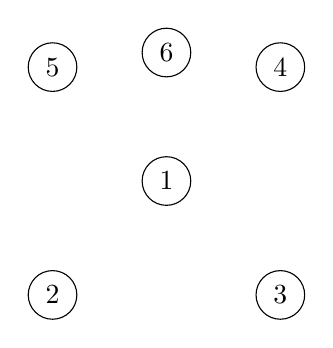
\begin{tikzpicture}[roundnode/.style = {circle, draw=black}]
     \node[roundnode] (1) {1};
     \node[roundnode] (2) [below left=of 1]{2};
     \node[roundnode] (3) [below right=of 1]{3};
     \node[roundnode] (5) [above left=of 1]{5};
     \node[roundnode] (4) [above right=of 1]{4};
     \node[roundnode] (6) [above=of 1]{6};
\end{tikzpicture}
\caption{Find the edges.}
\end{subfigure}
\end{figure}
\end{frame}
\begin{frame}{Problem- Cascades}
\begin{block}{Propagation Rules}
\begin{itemize}
    \item The infection is observed during a time window of length T,
    \item A vertex can only infect its neighbours,
    \item Once a vertex is infected it can not be infected again.
\end{itemize}
\end{block}
\begin{figure}
\begin{subfigure}{.4\textwidth}
    \centering
    \begin{tikzpicture}[roundnode/.style = {circle, draw=black}, infectednode/.style = {circle, draw=black, fill = green}]
     \node[roundnode] (1) {1};
     \only<4->\node[infectednode] (1) {1};
     \node[roundnode] (2) [below left=of 1]{2};
     \only<5-> \node[infectednode] (2) [below left=of 1]{2};
     \node[roundnode] (3) [below right=of 1]{3};
     \only<1>\node[roundnode] (5) [above left=of 1]{5};
     \only<2->\node[infectednode] (5) [above left=of 1]{5};
     \node[roundnode] (4) [above right=of 1]{4};
     \only<6->\node[infectednode] (4) [above right=of 1]{4};
     \node[roundnode] (6) [above=of 1]{6};
     \only<3->\node[infectednode] (6) [above=of 1]{6};
     \draw[->] (1)--(2);
     \only<5->\draw[thick,->] (1)--(2);
     \draw[->] (1)--(4);
     \only<6->\draw[thick,->](1)--(4);
     \draw[->] (2)--(5);
     \draw[->] (3)--(1);
     \draw[->] (3)--(2);
     \draw[->] (4)--(6);
     \draw[->] (5)--(6);
     \only<3->\draw[thick,->] (5)--(6);
     \draw[->] (6)--(1);
     \only<4->\draw[thick,->] (6)--(1);
\end{tikzpicture}
\end{subfigure}
\begin{subfigure}{.4\textwidth}
    \centering
    \begin{tikzpicture}[roundnode/.style = {circle, draw=black}, infectednode/.style = {circle, draw=black, fill = green}]
     \node[roundnode] (1) {1};
     \only<4->\node[infectednode] (1) {1};
     \node[roundnode] (2) [below left=of 1]{2};
     \only<5-> \node[infectednode] (2) [below left=of 1]{2};
     \node[roundnode] (3) [below right=of 1]{3};
     \only<1>\node[roundnode] (5) [above left=of 1]{5};
     \only<2->\node[infectednode] (5) [above left=of 1]{5};
     \node[roundnode] (4) [above right=of 1]{4};
     \only<6->\node[infectednode] (4) [above right=of 1]{4};
     \node[roundnode] (6) [above=of 1]{6};
     \only<3->\node[infectednode] (6) [above=of 1]{6};
     \only<3-> \draw[->] (5)--(6);
     \only<4-> \draw[->] (5)--(1);
     \only<4-> \draw[->] (6)--(1);
     \only<5-> \draw[->] (5)--(2);
     \only<5-> \draw[->] (6)--(2);
     \only<5-> \draw[->] (1)--(2);
     \only<6-> \draw[->] (5)--(4);
     \only<6-> \draw[->] (6)--(4);
     \only<6-> \draw[->] (1)--(4);
     \only<6-> \draw[round corner,->] (2)--(0,-1)--(4);
\end{tikzpicture}
\end{subfigure}
\end{figure}
\only<1>{$\textbf{t}^1$ = $(t_1,t_2,t_3,t_4,t_5,t_6)$}
\only<2> {$\textbf{t}^1$ = $(t_1,t_2,t_3,t_4,0,t_6)$}
\only<3> {$\textbf{t}^1$ = $(t_1,t_2,t_3,t_4,0,1)$}
\only<4> {$\textbf{t}^1$ = $(2,t_2,t_3,t_4,0,1)$}
\only<5> {$\textbf{t}^1$ = $(2,3,t_3,t_4,0,1)$}
\only<6> {$\textbf{t}^1$ = $(2,3,t_3,4,0,1)$}
\only<7> {$\textbf{t}^1$ = $(2,3,\infty,4,0,1)$ is called a \textit{cascade}}
\end{frame}
\begin{frame}{Problem formulation- Infectious rates}
\begin{block}{Definition}
To each pair of vertices $(i,j)$ a weight, $\alpha_{i,j} \geq 0$, corresponding to the infectious rate is associated. Let us denote the set of infectious rate by $\mathscr{A} = \{\alpha_{i,j}|(i,j)\in V \times V, i\neq j\}.$
\end{block}
\begin{block}{Remark}
\begin{itemize}
    \item There is an edge between node $i$ and node $j$ $\iff \alpha_{i,j} > 0$.
    \item The infectious parameter might be dynamic with respect to time, i.e $\alpha_{i,j} \leadsto \alpha_{i,j}(t)$.
\end{itemize}
\end{block}
\end{frame}
\begin{frame}{Problem formulation}
\begin{block}{Problem 1- Discrete optimization}
Given a collection of cascade $C$ propagating over a set of vertices $V$, find the underlying network $G^*$.
\end{block}
\begin{block}{Problem 2- Continuous optimization}
Given a collection of cascade $C$, find the correct infection parameters set $\mathscr{A}$.  
\end{block}
\begin{figure}
    \centering
    \includegraphics[scale = 0.1]{Detective_Pikachu_-_Character_artwork_01.png}
\end{figure}
\end{frame}

\section{Related work}
\begin{frame}{Frame Title}
    
\end{frame}
\section{New algorithm}
\section{Results}
\section{Conclusion}
\end{document}
